	\begin{center}
		\section{梦的开始}
	\end{center}

	\subsection{ASCII表}
	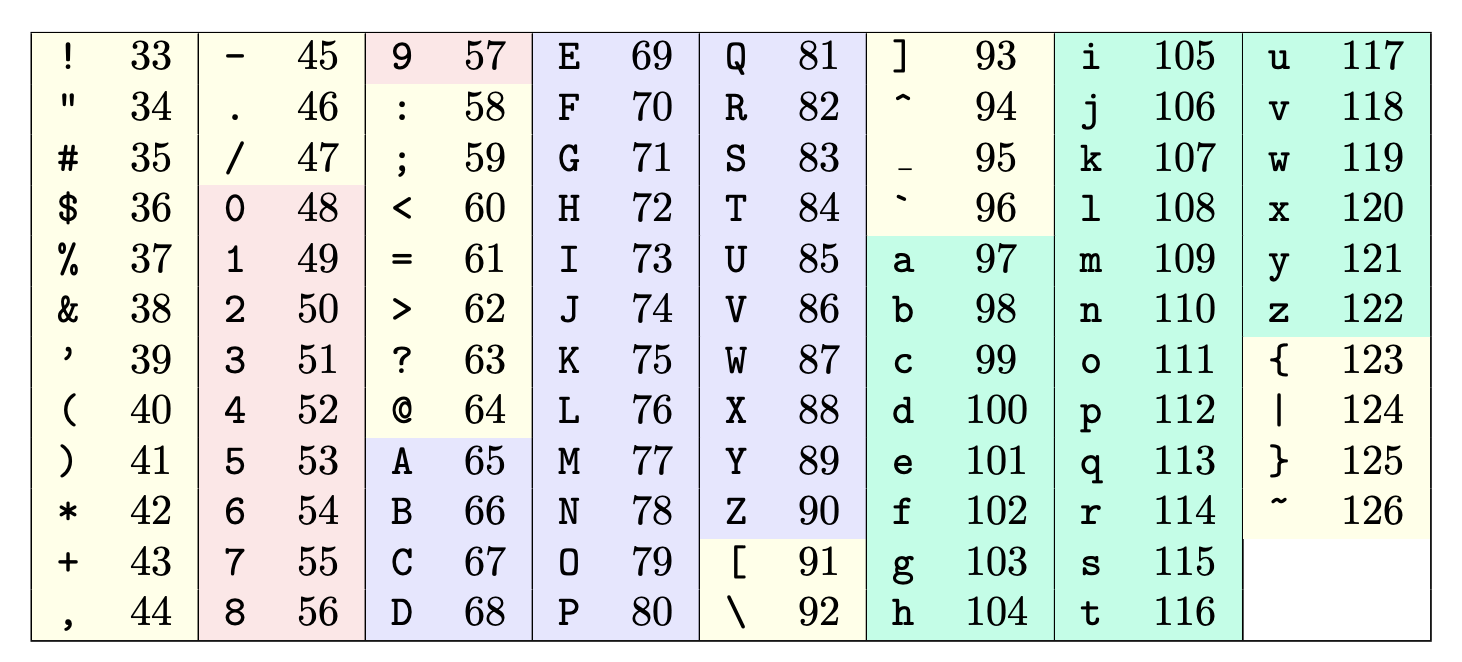
\includegraphics[width=\linewidth]{ASCII.png}

	\begin{multicols*}{2} % 开始双栏，数字 2 表示分两栏

		\subsection{初始化模板}

		\begin{minted}{cpp}
// teamname: Gospel_rock
/**
 * Problem: ${PROBLEM_NAME}
 * Contest: ${PROBLEM_GROUP_NAME}
 * Judge: ${ONLINE_JUDGE_NAME}
 * URL: ${PROBLEM_URL}
 * Created: ${YEAR}-${MONTH}-${DAY} ${HOUR}:${MINUTE}:${SECOND}
 * Author: Gospel_rock
 * My blog: https://znzryb.com/
 * 
 * Powered by AutoCp https://github.com/Pushpavel/AutoCp
 */

#include <bits/stdc++.h>
#define all(vec) vec.begin(), vec.end()
#define lson(o) (o << 1)
#define rson(o) (o << 1 | 1)
#define SZ(a) ((long long)a.size())
#define fsp(x) fixed << setprecision(x)
#define debug(x) cerr << "[" << #x << "]" << ": " << x << "\n"
#define cend cerr << "\n---------------------------------------------------\n"
#define cEnd cerr << "\n***************************************************\n"

using namespace std;

using ll = long long;
using ull = unsigned long long;
using DB = long double;
using i128 = __int128;
using CD = complex<double>;

static constexpr ll MAXN = (ll)1e6 + 10, INF = (1ll << 61) - 1;
static constexpr ll mod = 998244353;  // (ll)1e9+7;
static constexpr double eps = 1e-8;
// 不用 M_PI: 后者是 POSIX 扩展, glibc <cmath> 严格模式会 undef
const long double PI = acosl(-1.0);

ll lT, testcase;

/*
 *
 */

ll N;

void Solve() {
	cin >> N;
}

signed main() {
	ios::sync_with_stdio(false);
	cin.tie(nullptr);
	cout.tie(nullptr);
#ifdef LOCAL
	cout.setf(ios::unitbuf); // 无缓冲流，方便我们调试
#endif

	cin >> lT;
	for (testcase = 1; testcase <= lT; ++testcase)
		Solve();
	return 0;
}

/*

*/
		\end{minted}

		这个 \texttt{debug(x)} 是简版宏：单参数、直接 \texttt{cerr << x}，要求 \texttt{x} 支持 \texttt{operator<<}（基本类型 / \texttt{string} 都 OK，\texttt{vector<T>} 等容器不能直接打）。不再做 \texttt{LOCAL/非 LOCAL} 切换——OJ 上 stderr 通常不影响判分，留着也无伤大雅；介意的话提交前手动把 \texttt{debug(...)} 行删了或包成 \texttt{\#ifdef LOCAL} 即可。容器调试请用 range-for 手写循环。

		\subsection{CMake 配置}

		\subsubsection{Sanitizer 小技巧}

		有些越界或未定义行为问题，仅开 \texttt{address} 不一定能完整暴露。实践中建议同时开启 \texttt{address + undefined}，并保留帧指针，方便定位调用栈。

		\begin{minted}[highlightlines={9,10}]{cmake}
cmake_minimum_required(VERSION 3.31)
project(Edu_CF_186)

set(CMAKE_CXX_STANDARD 20)

add_executable(Edu_CF_186 main.cpp)

add_compile_definitions(LOCAL)
add_compile_options(-fsanitize=address,undefined -fno-omit-frame-pointer)
add_link_options(-fsanitize=address,undefined)

# 这个不要随便启用，启用后可能 debug 示数不可信
# add_compile_definitions(_GLIBCXX_DEBUG)

add_executable(A_New_Year_String "src/A_New_Year_String.cpp")
add_executable(B_New_Year_Cake "src/B_New_Year_Cake.cpp")
add_executable(odt_callback_bench "speed test/odt_callback_bench.cpp")
target_compile_options(odt_callback_bench PRIVATE "SHELL:${CMAKE_CXX_FLAGS_RELEASE}")
		\end{minted}

		\subsubsection{Cmake Release 配置小技巧}

		这个写法的主要目的有两个：一是只给特定目标启用 \texttt{Release} 进行性能测试，二是避免在 GUI 里把全局配置切到 \texttt{Release} 后忘记切回 \texttt{Debug}，进而出现调试信息异常、断点行为不符合预期等问题。

		\begin{minted}{cmake}
add_executable(odt_callback_bench "speed test/odt_callback_bench.cpp")
target_compile_options(odt_callback_bench PRIVATE "SHELL:${CMAKE_CXX_FLAGS_RELEASE}")
		\end{minted}

		\subsection{本地手测时怎么发 EOF}

		本地跑 \mintinline{cpp}{while (cin >> x)} / \mintinline{cpp}{while (scanf("\%d",&x) != EOF)} 这类按 EOF 终止的 CP 代码，手动在终端输完样例后要发 EOF 让 stdin 关流，否则程序一直阻塞读不到末尾。**EOF 的发送键在不同系统/终端里不一样**：

		\begin{itemize}
			\item \textbf{macOS / Linux 真终端}：\texttt{Ctrl-D}（在空输入行上按）。
			\item \textbf{Windows \texttt{cmd} / PowerShell}：\texttt{Ctrl-Z} 后按 \texttt{Enter}。
			\item \textbf{WSL / Git Bash on Windows}：\texttt{Ctrl-D}（同 Unix）。
			\item \textbf{CLion / VSCode Run 控制台}：跟底层 shell 走，mac/Linux $\Rightarrow$ \texttt{Ctrl-D}，Windows $\Rightarrow$ \texttt{Ctrl-Z}+\texttt{Enter}。
		\end{itemize}

		\textbf{两个坑}：

		\begin{itemize}
			\item \texttt{Ctrl-D} 只有在\textbf{空输入行}上才发 EOF；当前行已经敲了字符时，\texttt{Ctrl-D} 只把缓冲 flush 一次，要再按一次才真关流。
			\item CLion / VSCode 内嵌的 Run / Debug 控制台不是真 TTY，有的版本不响应 \texttt{Ctrl-D}——这时改用文件重定向喂输入：\mintinline{bash}{./a.out < in.txt}，或者直接用 heredoc：

\begin{minted}{bash}
./a.out << 'EOF'
3
1 2 3
EOF
\end{minted}
		\end{itemize}

	\end{multicols*} % 结束双栏

	\subsection{CLion 常用功能与快捷键（默认 keymap）}

	赛场 / 平时最常用的几个 CLion 操作与默认快捷键如下（赛场机一律 Windows / Linux，故只列这一套绑定）。\textbf{Run context configuration} 指「运行光标当前所在的那个目标」——多目标 CMake 工程里免去手动切下拉框，直接跑当前打开的这道题；\textbf{Reformat Code} 是一键格式化当前文件 / 选区；\textbf{Rename} 是语义级重命名，改变量 / 函数名时所有引用一起改，比全文替换安全（不会误伤字符串和同名的别的符号）。快捷键随 keymap 版本略有出入，忘了就用 \textbf{Find Action}（\texttt{Ctrl+Shift+A}）搜功能名，弹出项右侧直接显示当前绑定。

	\begin{center}
		\begin{tabular}{l|l}
			\hline
			功能 & Windows / Linux \\
			\hline
			Run context configuration（跑光标所在目标） & \texttt{Ctrl+Shift+F10}    \\
			\hline
			Run（当前选中的配置）                       & \texttt{Shift+F10}         \\
			\hline
			Debug（当前选中的配置）                     & \texttt{Shift+F9}          \\
			\hline
			Build Project（只编译不跑）                 & \texttt{Ctrl+F9}           \\
			\hline
			Reformat Code（格式化当前文件 / 选区）       & \texttt{Ctrl+Alt+L}        \\
			\hline
			Rename（重命名符号 + 所有引用）              & \texttt{Shift+F6}          \\
			\hline
			注释 / 取消注释行                           & \texttt{Ctrl+/}            \\
			\hline
			复制当前行 / 选区                           & \texttt{Ctrl+D}            \\
			\hline
			删除整行                                   & \texttt{Ctrl+Y}            \\
			\hline
			上 / 下移当前行                            & \texttt{Alt+Shift+Up/Down} \\
			\hline
			Find Action（搜任意功能 / 快捷键）           & \texttt{Ctrl+Shift+A}      \\
			\hline
		\end{tabular}
	\end{center}

	\subsection{CLion 语言引擎：赛场机上先切 Nova}

	CLion 有两套\textbf{语言引擎}，补全 / 高亮 / 跳转的行为由它决定，**赛场机开机后第一件事就是确认切到 Nova**：

	\begin{itemize}
		\item \textbf{CLion Classic}——核心 code insight（补全、高亮）由 \textbf{clangd} 提供，另有一个 legacy 引擎负责重构等其余功能。
		\item \textbf{CLion Nova}——换成 \textbf{ReSharper C++ / Rider C++ 引擎}，核心功能\textbf{完全不走 clangd}（JetBrains 的 clangd fork 仍在后台跑，但只管 ClangFormat / Clang-Tidy / MISRA / 数据流分析）。
	\end{itemize}

	两套是彼此独立的实现，所以「同一个 IDE、同一份代码，两台机补全行为不一样」很正常——换引擎等于换了整个语言前端。对竞赛影响最大的一处差异：

	\begin{center}
		\begin{tabular}{l|l|l}
			\hline
			输入                                & CLion Nova                                     & CLion Classic                        \\
			\hline
			\mintinline{cpp}{vec} + \texttt{Enter}  & \mintinline{cpp}{vector<>}（光标落在尖括号中间） & \mintinline{cpp}{vector}（尖括号自己敲） \\
			\hline
			\mintinline{cpp}{#inc} + \texttt{Enter} & \mintinline{cpp}{#include}（只有指令）           & \mintinline{cpp}{#include <>} + 头文件列表 \\
			\hline
		\end{tabular}
	\end{center}

	第一行是\textbf{选 Nova 的主要理由}：竞赛里 \mintinline{cpp}{vector} / \mintinline{cpp}{map} / \mintinline{cpp}{priority_queue} 满屏都是，少敲一对尖括号累积起来很可观。Classic 这边\textbf{既不是 bug 也没有开关}——clangd 只对\textbf{函数模板}（且模板参数推导不出来时）补尖括号，\textbf{类模板一律不补}：C++17 起有了 CTAD，\mintinline{cpp}{vector v{1, 2};} 本身就合法，IDE 判断不出你要不要那对尖括号，索性不插（见 JetBrains issue \texttt{CPP-154}）。

	第二行是反向的坑，切之前知道一下：Nova 目前\textbf{没有} \mintinline{cpp}{#include <...>} 的补全，只补一个光秃秃的 \mintinline{cpp}{#include}（issue \texttt{CPP-47569}，仍 open）。竞赛基本只写一行 \mintinline{cpp}{#include <bits/stdc++.h>}，影响不大。

	\textbf{怎么切}（两条路径任选其一）：

	\begin{enumerate}
		\item 右侧工具栏齿轮（\textbf{IDE and Project Settings}）$\rightarrow$ \textbf{Switch to Nova Engine} $\rightarrow$ \textbf{Enable and Restart}。
		\item \textbf{Settings} $\rightarrow$ \textbf{Advanced Settings} $\rightarrow$ 勾上 \textbf{Use the ReSharper C++ language engine (CLion Nova)} $\rightarrow$ \textbf{Apply}。
	\end{enumerate}

	切换要重启 IDE 并重新解析项目。竞赛工程就几个 \texttt{.cpp}，几秒的事，但\textbf{务必在热身赛就切好}，别等开赛才发现要重启。IDE 设置是每台机独立的，赛场机每次重装镜像都要重切一次。

	\textbf{版本背景}：Nova 自 \textbf{CLion 2025.3} 起是所有用户的默认引擎；\textbf{2026.2} 把 Classic 从 IDE 里 unbundle 成可选插件（\texttt{C/C++ Language Support via Classic Engine}）；\textbf{2026.3}（2026 年 11 月）是最后一个兼容 Classic 的稳定版。所以赛场机若装了较新版本，默认就是 Nova、无需操心；只有还能看到「选不选 Nova」的机器（版本大致在 2024.2--2026.1 之间）才需要手动切。

	\subsection{Windows：禁用 \texttt{Shift} 切换中英文输入}

	Windows 赛场机上敲代码，误碰 \texttt{Shift}（打大写、打符号松手稍慢）就会被输入法切到中文模式，接着敲出一串全角字符——开赛前先把这个切换键关掉。

	\subsubsection{微软拼音（系统自带，Win10 逐步截图）}

	\begin{enumerate}
		\item 开始菜单 → \textbf{设置}：
		      \begin{center}
			      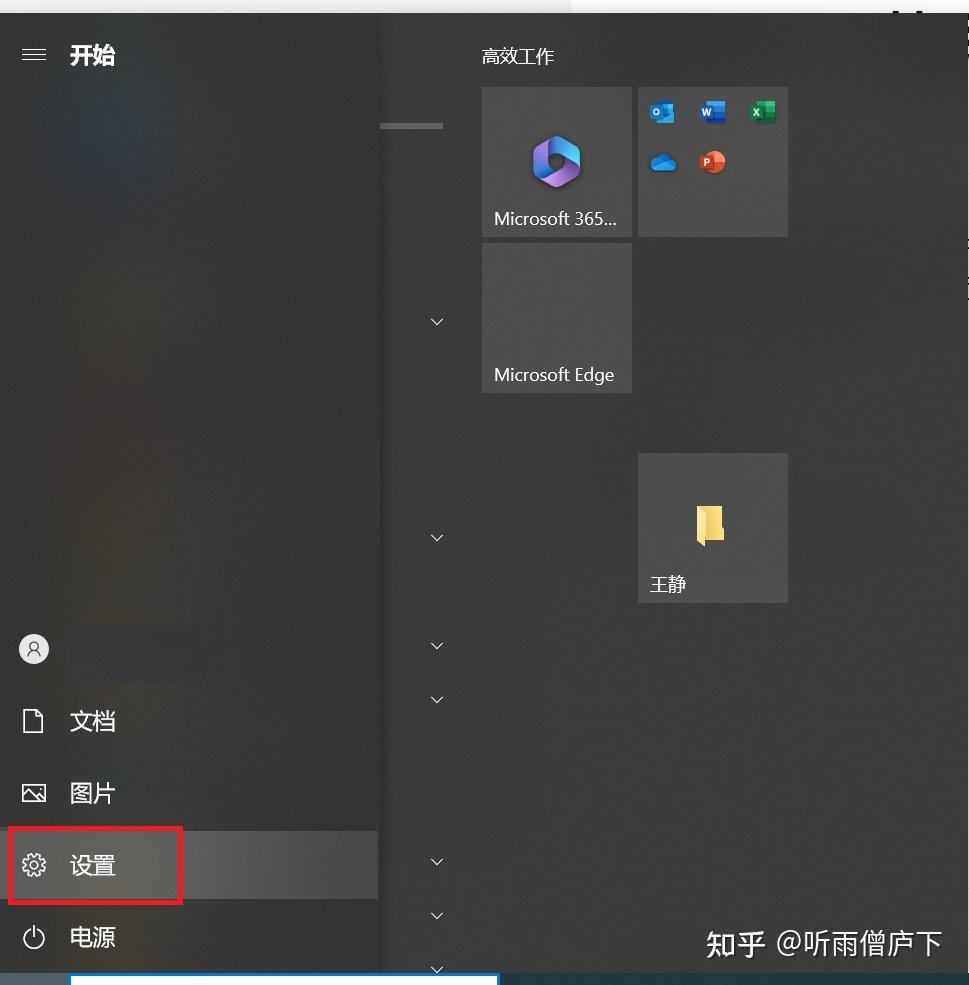
\includegraphics[width=0.42\linewidth]{image/ime_win10_01_开始菜单设置.jpg}
		      \end{center}
		\item 进入\textbf{时间和语言}：
		      \begin{center}
			      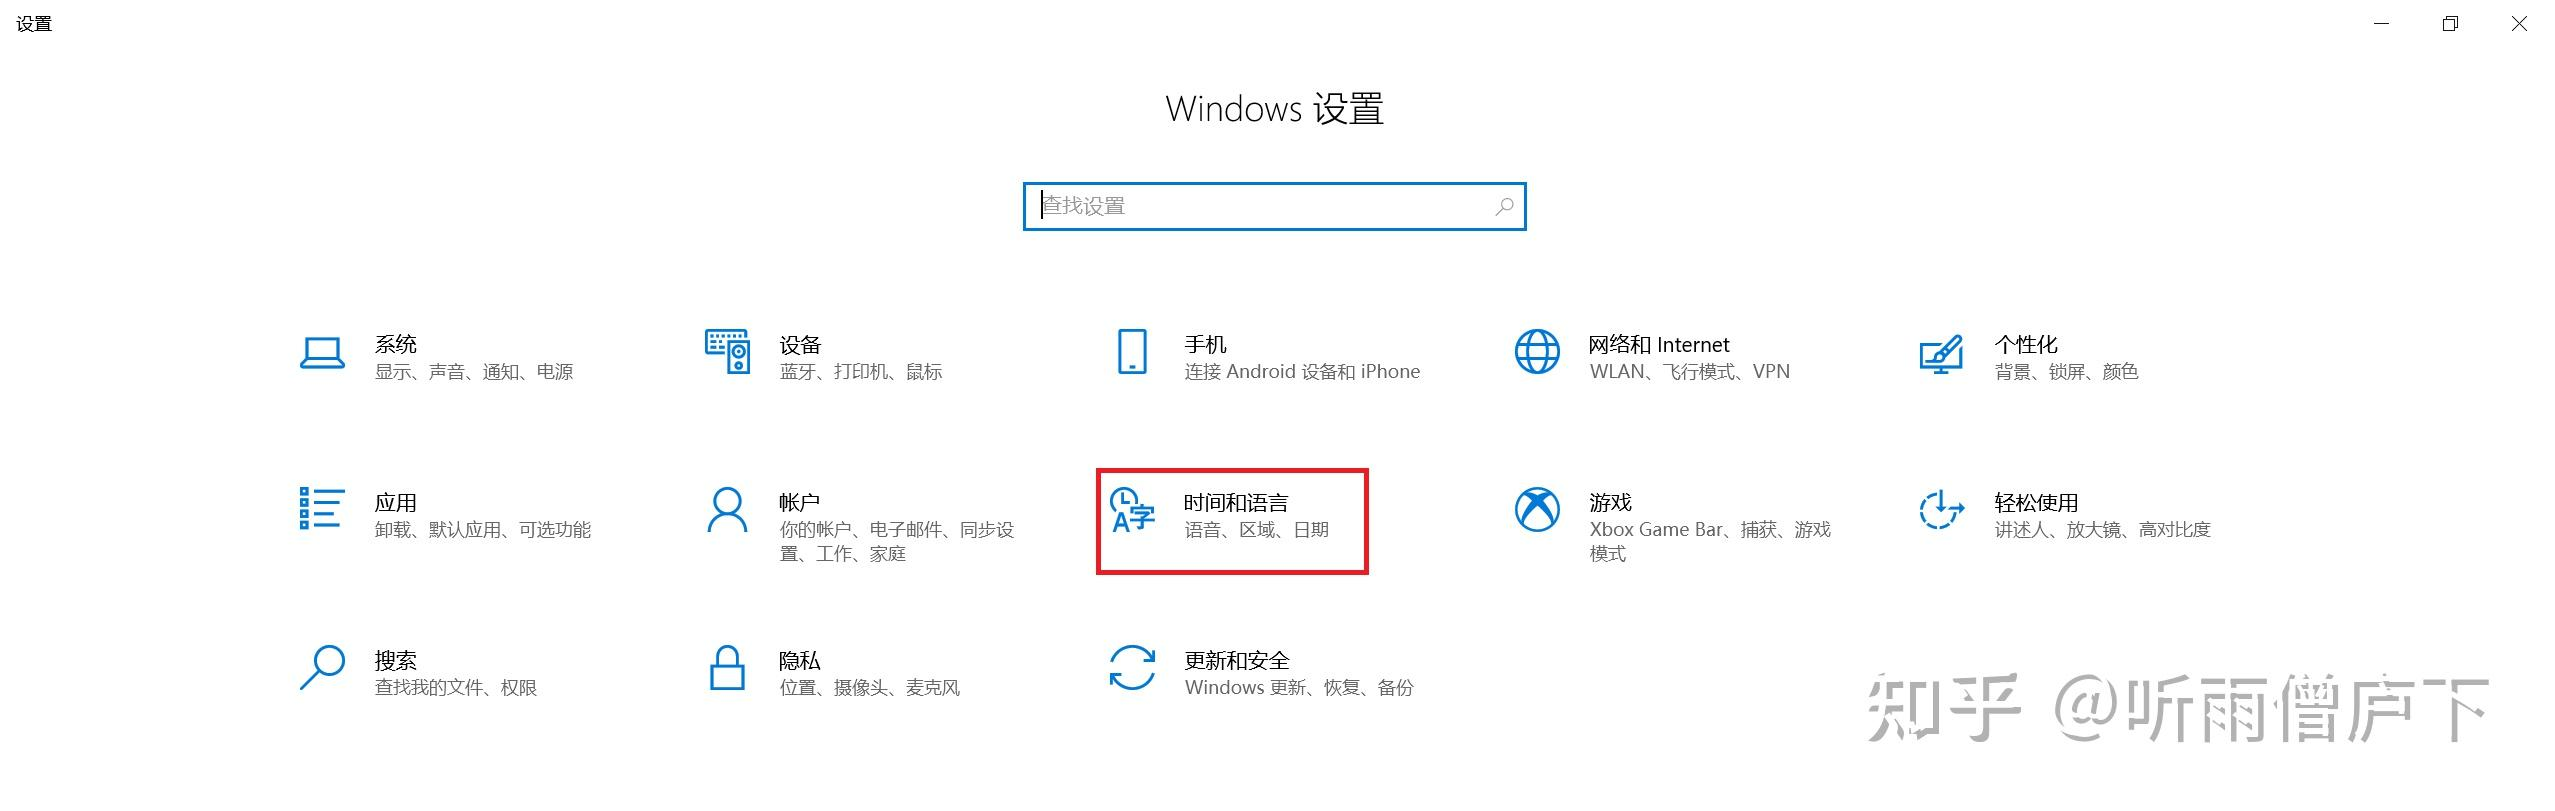
\includegraphics[width=0.85\linewidth]{image/ime_win10_02_时间和语言.jpg}
		      \end{center}
		\item 左侧栏切到\textbf{语言}：
		      \begin{center}
			      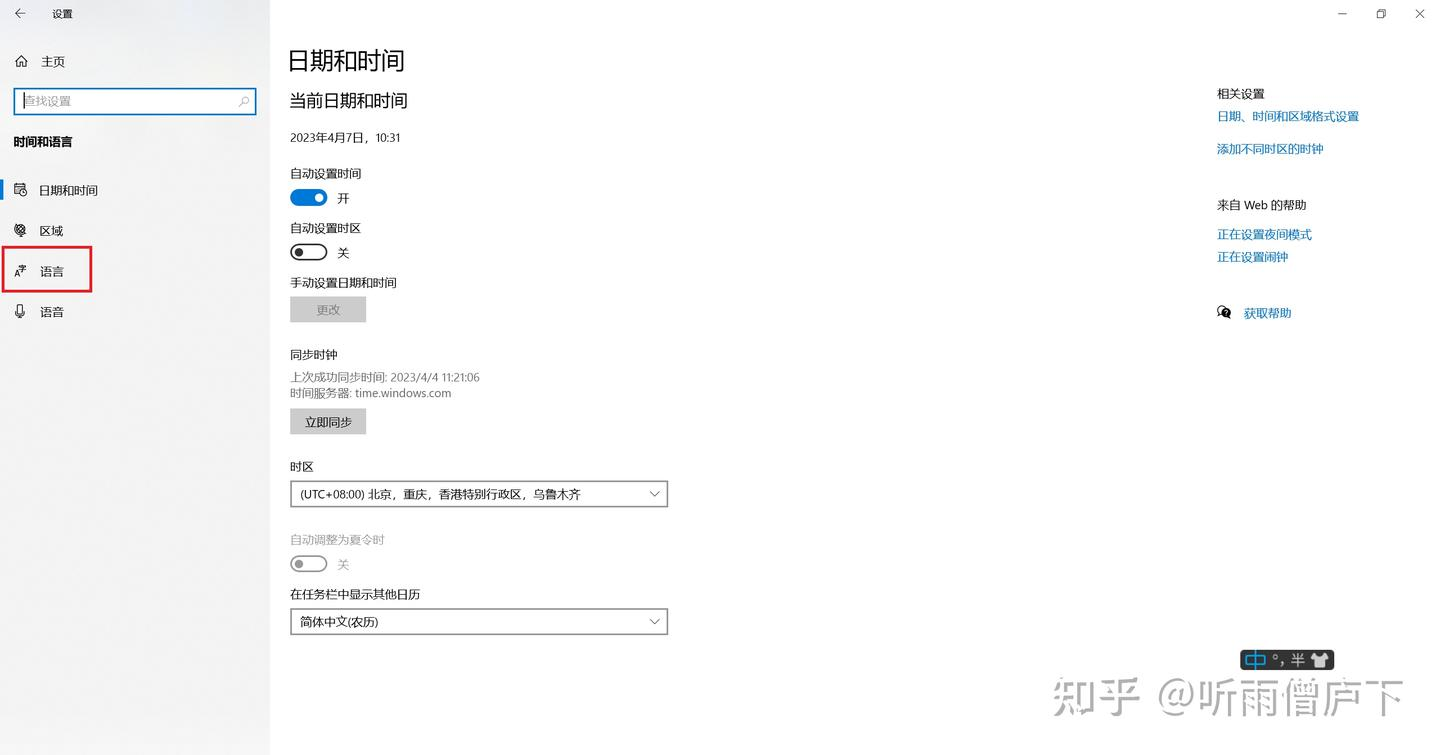
\includegraphics[width=0.75\linewidth]{image/ime_win10_03_左栏语言.jpg}
		      \end{center}
		\item 「首选语言」列表里点\textbf{中文(简体，中国)}：
		      \begin{center}
			      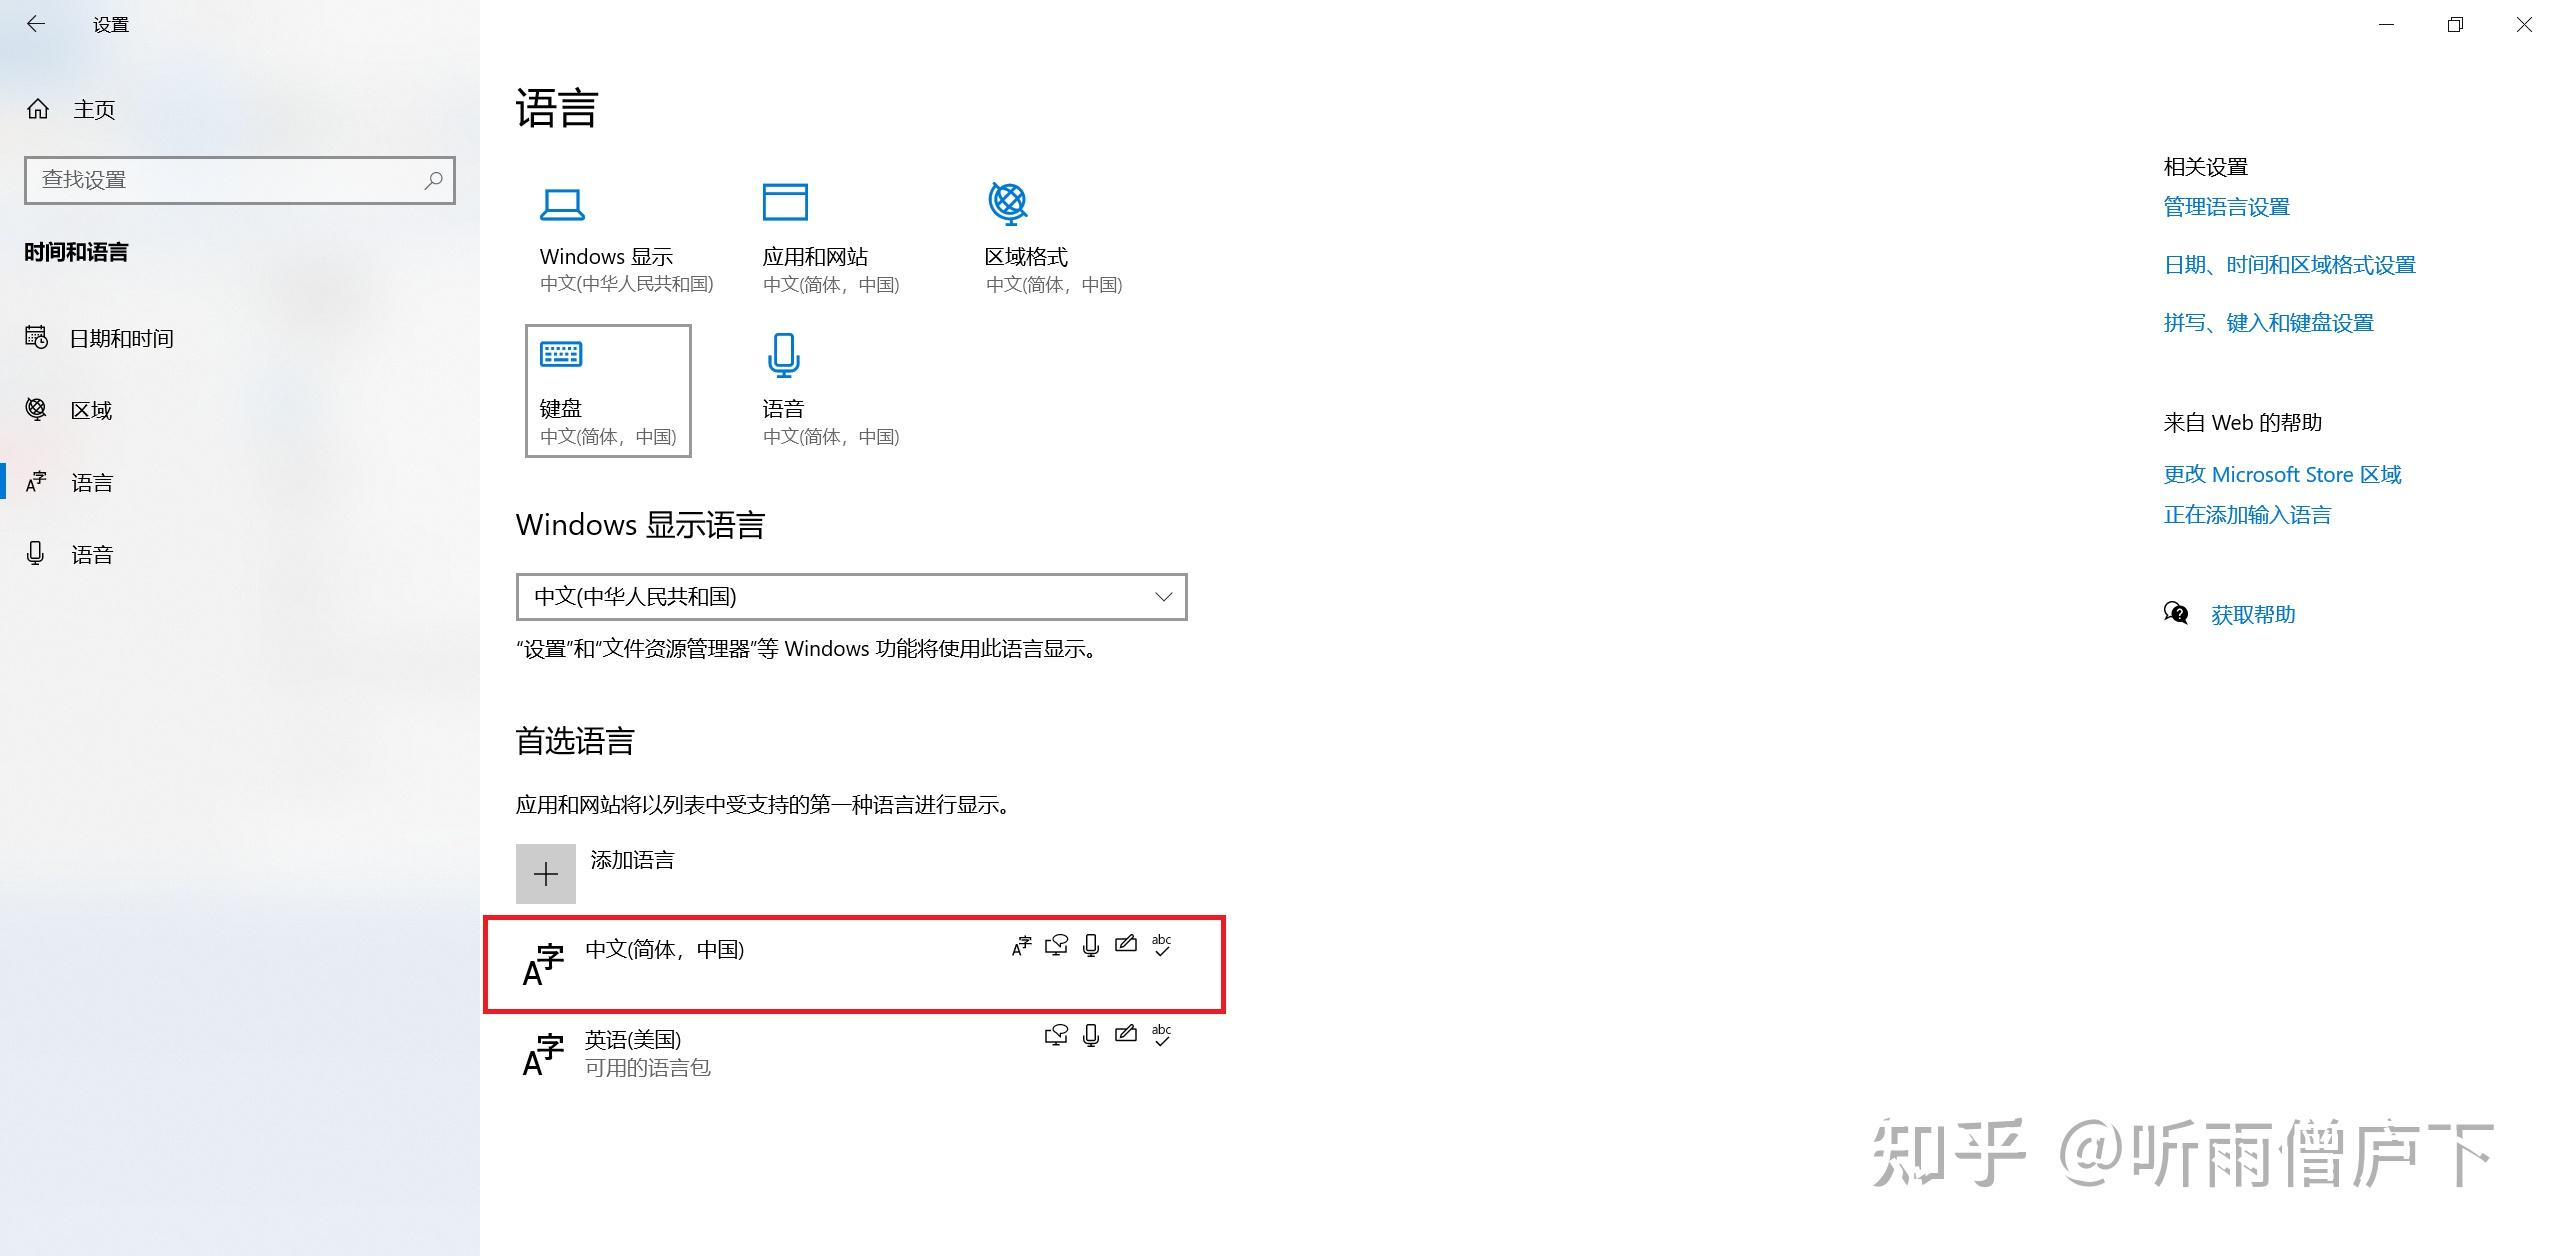
\includegraphics[width=0.85\linewidth]{image/ime_win10_04_首选语言点中文.jpg}
		      \end{center}
		\item 点展开出来的\textbf{选项}按钮：
		      \begin{center}
			      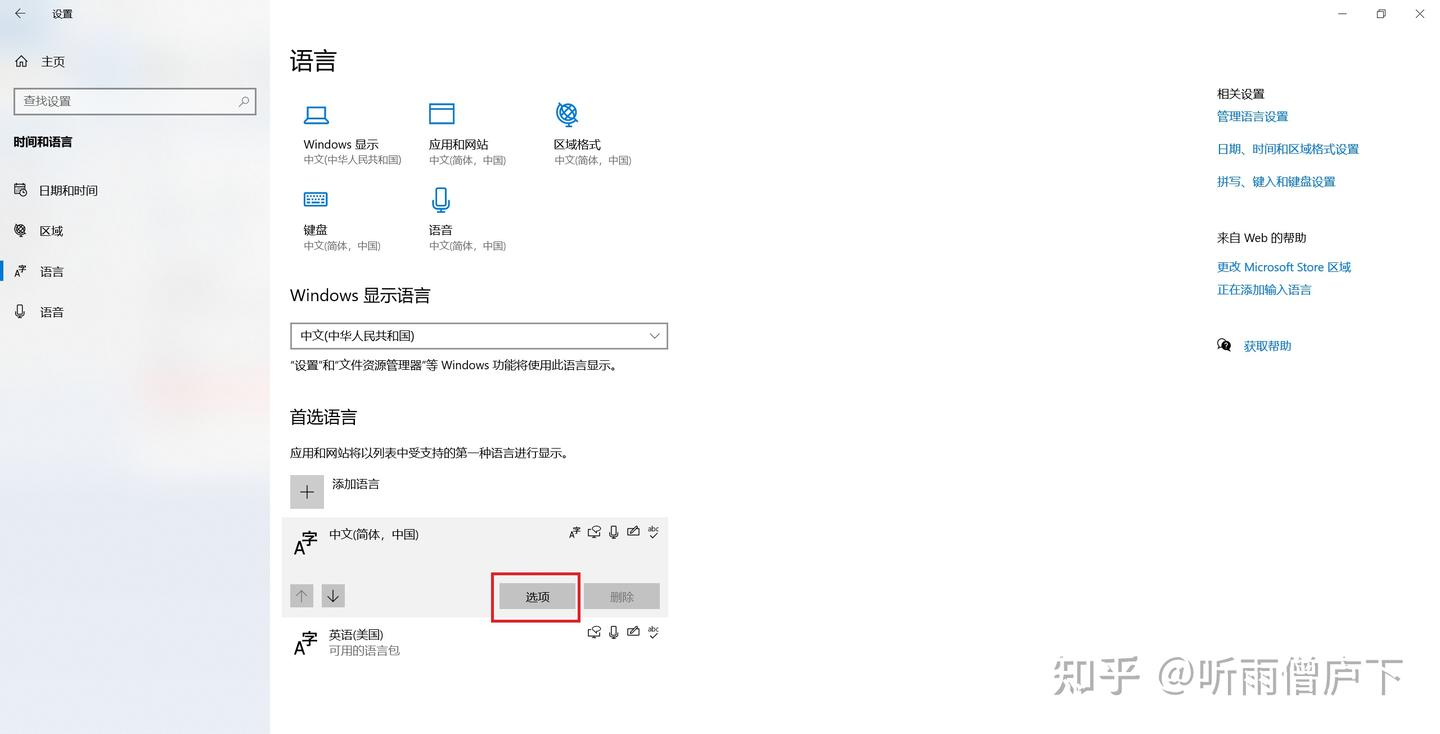
\includegraphics[width=0.75\linewidth]{image/ime_win10_05_选项按钮.jpg}
		      \end{center}
		\item 键盘列表里点\textbf{微软拼音} → 进入\textbf{按键}：
		      \begin{center}
			      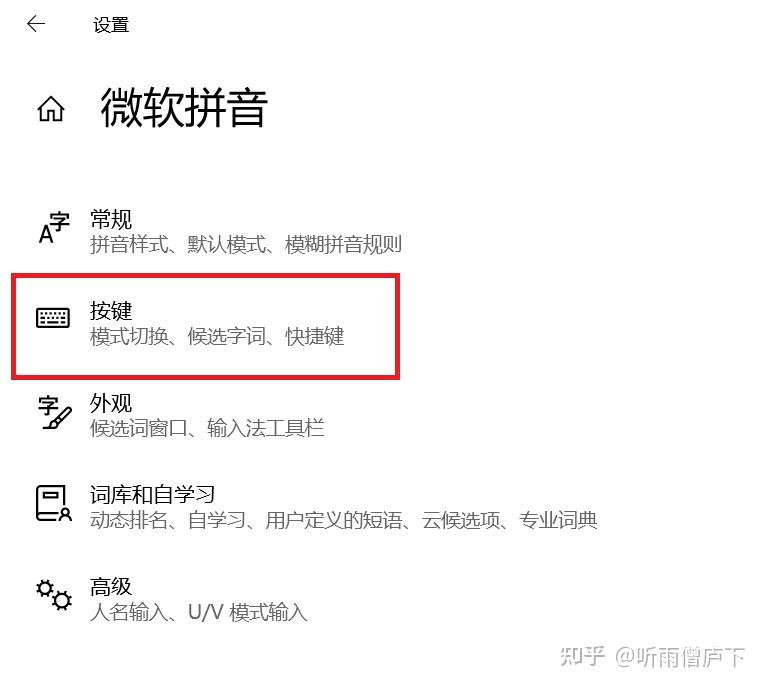
\includegraphics[width=0.45\linewidth]{image/ime_win10_06_微软拼音按键.jpg}
		      \end{center}
		\item 「中/英文模式切换」里\textbf{把 \texttt{Shift} 的勾去掉}（保留 \texttt{Ctrl + 空格键}，这就是之后手动切中英文的键）：
		      \begin{center}
			      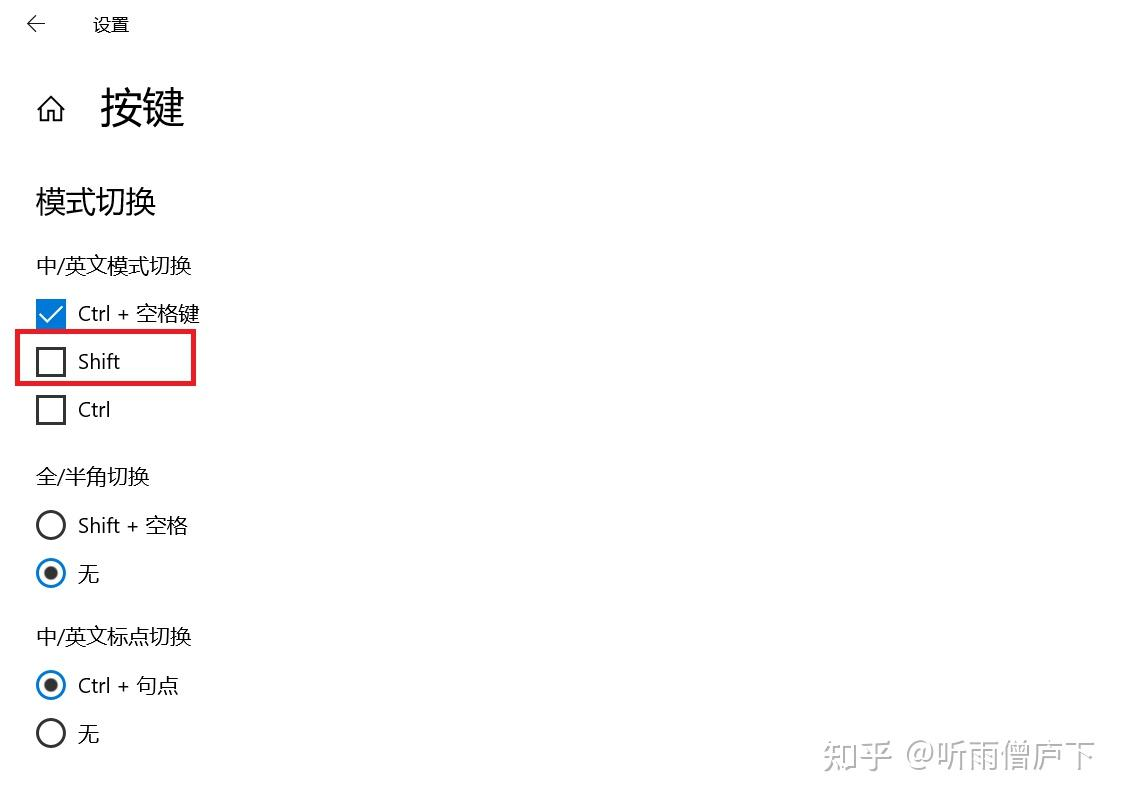
\includegraphics[width=0.55\linewidth]{image/ime_win10_07_取消Shift勾选.jpg}
		      \end{center}
	\end{enumerate}

	改完后 \texttt{Shift} 只做普通修饰键；切中英文用 \texttt{Ctrl + Space}，切输入法 / 语言用 \texttt{Win + Space}。Win11 路径名稍有不同：设置 → 时间和语言 → \textbf{语言和区域} → 中文右侧「…」→ 语言选项 → 微软拼音 → 键盘选项 → 按键，最后一步相同。

	\subsubsection{搜狗输入法}

	\begin{enumerate}
		\item 任务栏搜狗图标打开工具面板 → \textbf{更多设置(P)}：
		      \begin{center}
			      
\includegraphics[width=0.3\linewidth]{image/ime_sogou_01_更多设置.jpg}
		      \end{center}
		\item 属性设置 → \textbf{按键} → 「中英切换」选\textbf{无}（不想彻底禁可选 \texttt{Ctrl}）：
		      \begin{center}
			      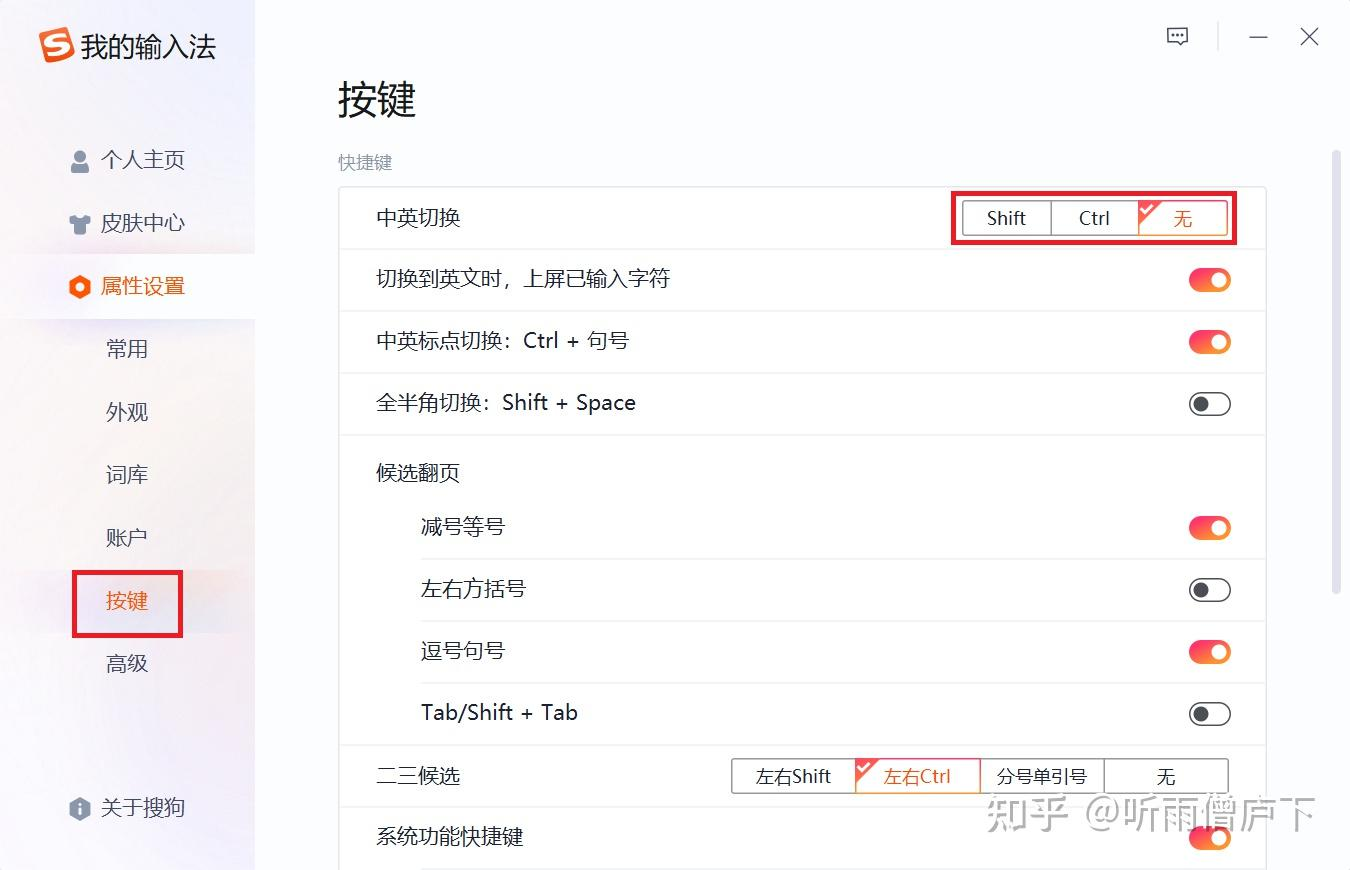
\includegraphics[width=0.6\linewidth]{image/ime_sogou_02_中英切换选无.jpg}
		      \end{center}
	\end{enumerate}

	QQ / 百度输入法路径类似，都在「按键设置」里。

	\textbf{更省事的做法}（比赛全程不需要中文输入时）：直接在上面第 4 步的语言列表里\textbf{删掉中文输入法}或把默认语言切到 \texttt{ENG}，\texttt{Shift} 就完全没有切换语义了。快速定位入口：开始菜单搜「输入法」→「编辑语言和键盘选项」。





